\section{Решение задачи}

\subsection{Перцептрон}
	Перцептрон состоит из нескольких слоёв нейронов:
	\begin{enumerate}
		\item Входной слой, содержащий псевдо-нейроны, которые передают дальше значения \textit{предикторов}~--- параметров объекта;
		\item Один или несколько скрытых слоёв;
		\item Выходной слой, содержащий один нейрон.
	\end{enumerate}

	Передача сигналов (активация) нейронной сети происходит от входного слоя, через скрытые слои, к выходному слою.
	\parskip=0cm
	
	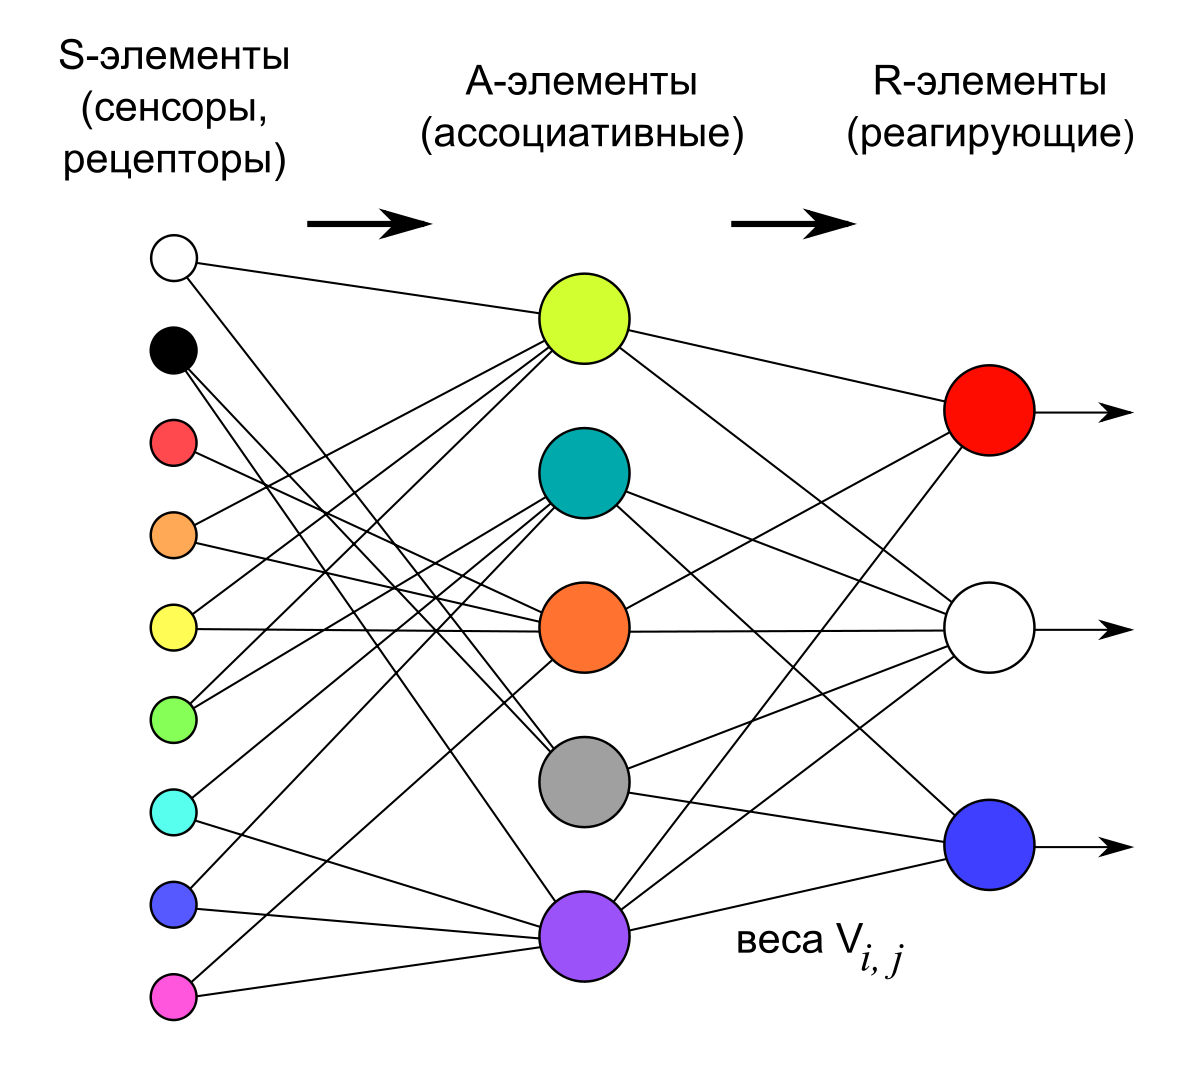
\includegraphics[width=450px, height=370px]{picture1.png}
	\parskip=0.2cm

	Все нейроны (кроме входного слоя) имеют одинаковое строение, состоят из двух частей~--- сумматорной и активационной функций.
	Сумматорная функция определяет то, как нейрон будет использовать входящую информацию из предыдущего слоя.
	Активационная функция определяет реакцию нейрона, которая будет передана по всем выходным связям в следующий слой.

	В качестве сумматорной функции выбрана взвешенная сумма всех входящих сигналов:
	\[
		S = b + \sum_{j = 1}^m x_j w_j
	\]
	где $m$~--- количество входящих сигналов нейрона, $x_j$~--- значение, получаемое по $j$-ому входу, $w_j$~--- вес $j$-ого входа,
	$b$~--- некоторое смещение, изменяемое в процессе обучения.	Смещение можно учитывать в сумме,
	если добавить в каждый слой, кроме выходного на первое место нейрон, у которого значение активации будет всегда равно 1.

	Активационная функция~--- логистическая (сигмоидальная):
	\[
		\sigma\left(S\right) = \frac{1}{1 + e^{-S}}
	\]
	\parskip=0cm

	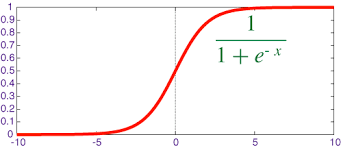
\includegraphics[width=400px]{picture2.png}
	\parskip=0.2cm

	Логистическая функция является гладкой, что необходимо для работы алгоритма обучения. Кроме того, её значение можно
	интерпретировать как вероятность принадлежности объекта к одному из двух классов.

	\textit{Обучение нейронной сети}~--- это настройка весов для входящих связей всех нейронов, с целью получения достоверных предсказаний.
	Для обучения используется \textit{алгоритм обратного распространенния ошибки}, который основывается на градиентном спуске по простанству
	весов в сторону уменьшения значений целевой функции ошибки.

	Для оценки правдоподобности предсказаний используется \textit{квадратичная функция ошибки}:
	\[
		E = \frac{1}{2N}\sum_{i = 1}^N \left(\hat y_i - y_i\right)^2
	\]
	где $N$~--- количество примеров, $\hat y_i$~--- предсказанное значение для $i$-ого примера, $y_i$~--- правильный ответ для него.

	Для того, чтобы понять, как изменится значение функции ошибки при изменении какого-либо веса входящих сигналов нейрона,
	нужно взять её частную производную по этому весу.

	Сначала считается изменение весов в выходном слое:
	\[
		\Delta w_j = -\alpha\frac{\partial E}{\partial w_j}
	\]
	где $\alpha \in \mathbb R$~--- скорость обучения.

	В векторном виде:
	\[
		\Delta W = -\alpha\nabla_W E
	\]
	где $\nabla_W E = \left(\frac{\partial E}{\partial w_1},\dots,\frac{\partial E}{\partial w_m}\right)$~--- градиент $E$ в точке $W$.

	Посчитаем частную производную от функции $E$ по $j$-му весу:
	\[
		\frac{\partial E}{\partial w_j}	= \frac{\partial\left(\frac{1}{2N}\sum_{i = 1}^N \left(\hat y_i - y_i\right)^2\right)}{\partial w_j}
	\]
	
	Так как производная суммы равна сумме производных, возьмём для простоты один пример, а после просуммируем все значения:
	\[
		\frac{1}{2}\cdot\frac{\partial{\left(\hat y - y\right)^2}}{\partial w_j} =
		\frac{1}{2}\cdot\frac{\partial\left(\hat y - y\right)^2}{\partial\hat y}\cdot\frac{\partial\hat y}{\partial w_j} =
		\left(\hat y - y\right)\frac{\partial\sigma\left(S\right)}{\partial w_j} =
	\]
	\[
		= \left(\sigma\left(S\right) - y\right)\sigma\prime\left(S\right)\frac{\partial\sum_{j = 1}^m x_j w_j}{\partial w_j} =
		\left(\sigma\left(S\right) - y\right)\sigma\left(S\right)\left(1 - \sigma\left(S\right)\right) x_j
	\]

	Итак, общая формула для $j$-ого веса по $N$ примерам:
	\[
		\frac{\partial E}{\partial w_j} = \frac{1}{N}\sum_{i = 1}^N
		\left(\hat y_i - y_i\right)\hat y_i\left(1 - \hat y_i\right) x_j
	\]

	Далее полученная ошибка распространяется по ИНС в обратном порядке, от выходного слоя ко входному, изменяя веса скрытых слоёв.
	
	Введём следующие обозначения:
	\begin{itemize}
		\item $w_{jk}^l$~--- значение $j$-ого веса $k$-ого нейрона в $l$-ом слое (вес связи из $j$-ого нейрона $l - 1$ слоя в $k$-ый нейрон $l$-ого слоя);
		\item $m_l$~--- количество нейронов в $l$-ом слое;
		\item $s_k^l$~--- значение сумматорной функции $k$-ого нейрона в $l$-ом слое;
		\item $a_k^l$~--- значение активационной функции $k$-ого нейрона в $l$-ом слое;
		\item $\delta_k^l = \frac{\partial E}{\partial s_k^l}$~--- ошибка $k$-ого нейрона в $l$-ом слое.
	\end{itemize}

	Зная значение ошибки $\delta_k^l$ для каждого нейрона, можно получить соответствующее изменение его весов:
	\[
		\Delta w_{jk}^l = -\alpha\delta_k^l a_j^{l-1}
	\]

	Посчитаем значение ошибки для нейронов выходного ($L$-ого) слоя. Для простоты возьмём один пример:
	\[
		\delta_k^L = \frac{\partial E}{\partial s_k^L} =
		\frac{1}{2}\cdot\frac{\partial\left(\sigma\left(s_k^L\right) - y_k\right)^2}{\partial s_k^L} = 
		\left(a_k^L - y_k\right)a_k^L\left(1 - a_k^L\right)
	\]
	где $y_k$~--- правильный ответ для $k$-ого нейрона выходного слоя.

	Теперь выразим ошибку нейрона на $l$-ом слое через ошибки на $l + 1$ слое:
	\[
		\delta_j^l = \sigma\prime\left(s_j^l\right)\sum_{k = 1}^{m_{l + 1}} w_{jk}^{l + 1} \delta_k^{l+1} = 
		a_j^l\left(1 - a_j^l\right)\sum_{k = 1}^{m_{l + 1}} w_{jk}^{l + 1} \delta_k^{l+1}
	\]

\subsection{Предикторы}
	Для получения численных предикторов вычисляется рассояние от точки движения до прямых ограждающих трассу.В каждый момент поворота есть вектор предыдущего движения и по два вектра в разные стороны от него. Значения длин отрезков по этим пяти векторам и есть предикторы.
	
	Естественноучитывается только расстояние до ближайшей стенки(если прямая ,заданная вектором, пересекает несколько "стенок",то берется кратчайший путь).